%!TEX root = ../paper.tex
We compare the performance of the shape-adaptive method with that of the Modified Breiman Estimator. \Cref{ss:3:datasets} introduces the datasets used in our experiments. The metrics used to compare the performance of the different estimators are introduced in \cref{ss:3:errorMeasures}.

\subsection{Datasets}
\label{ss:3:datasets}
	The performance of the estimators is investigated with two groups of datasets: a number of simulated datasets with known density fields and a real world dataset with an unknown density field. The simulated datasets allow us to test how well a method can recover simple density distributions. Whereas the real world dataset makes it possible to compare the performance of the estimators in the context in which they would be applied. 

	\subsubsection*{Simulated Datasets}
	%!TEX root = ../paper.tex

The simulated datasets are a superset of the sets used by \textcite{ferdosi2011comparison}. \Cref{fig:3:simulated:datasets} shows scatter plots of these sets, their definition is given in \cref{tab:3:simulated:datasets}.

\begin{figure*}
	\centering
	\beforeFinalVersion{Remove ticks and labels.}
	%!TEX root = ../paper.tex
%Ferdosi Sets 1/3
\begin{subfigure}{0.23\textwidth}
	\centering
	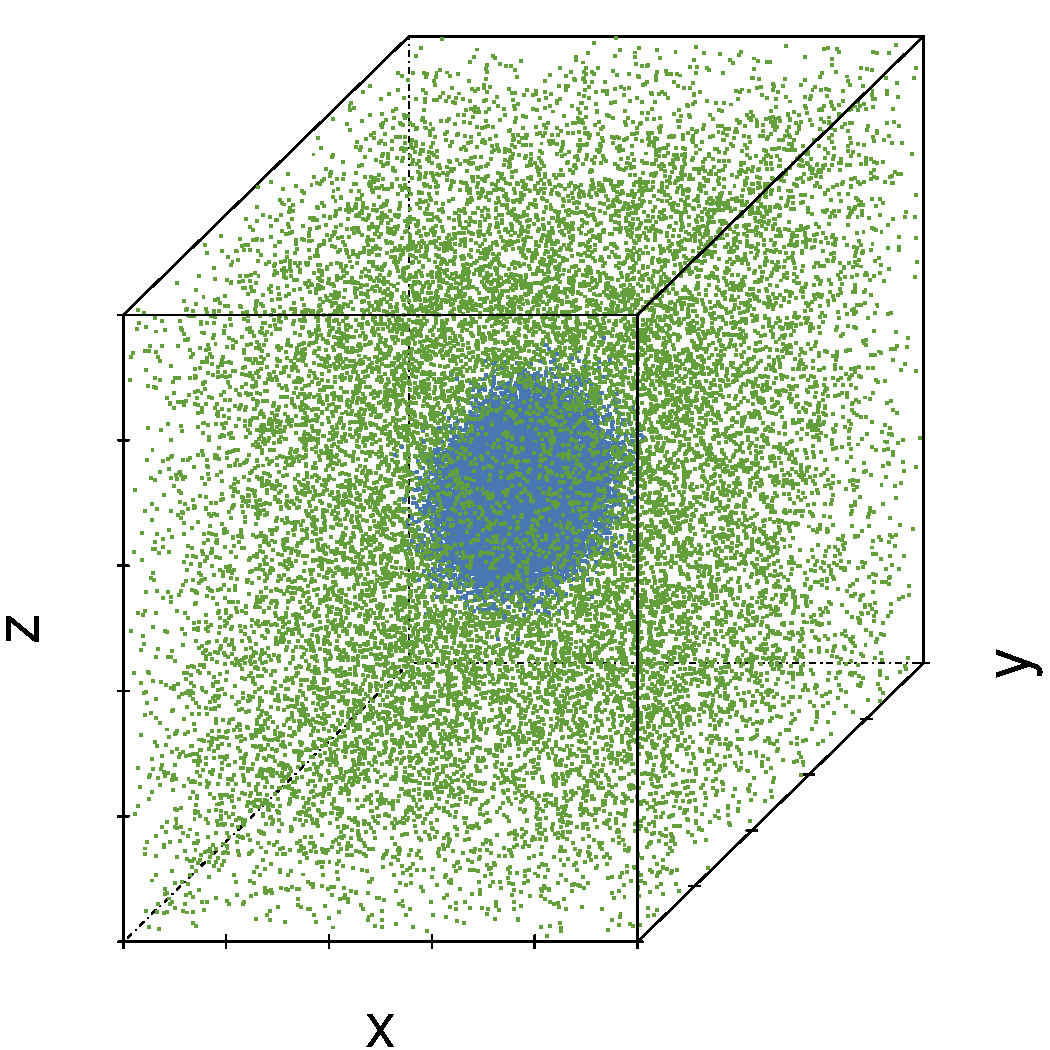
\includegraphics[width=\textwidth]{3/img/datasetplot_ferdosi_1_60000.pdf}
	\caption{Set \ferdosiOne}
	\label{fig:3:simulated:datasets:ferdosi1}
\end{subfigure}
\begin{subfigure}{0.23\textwidth}
	\centering
	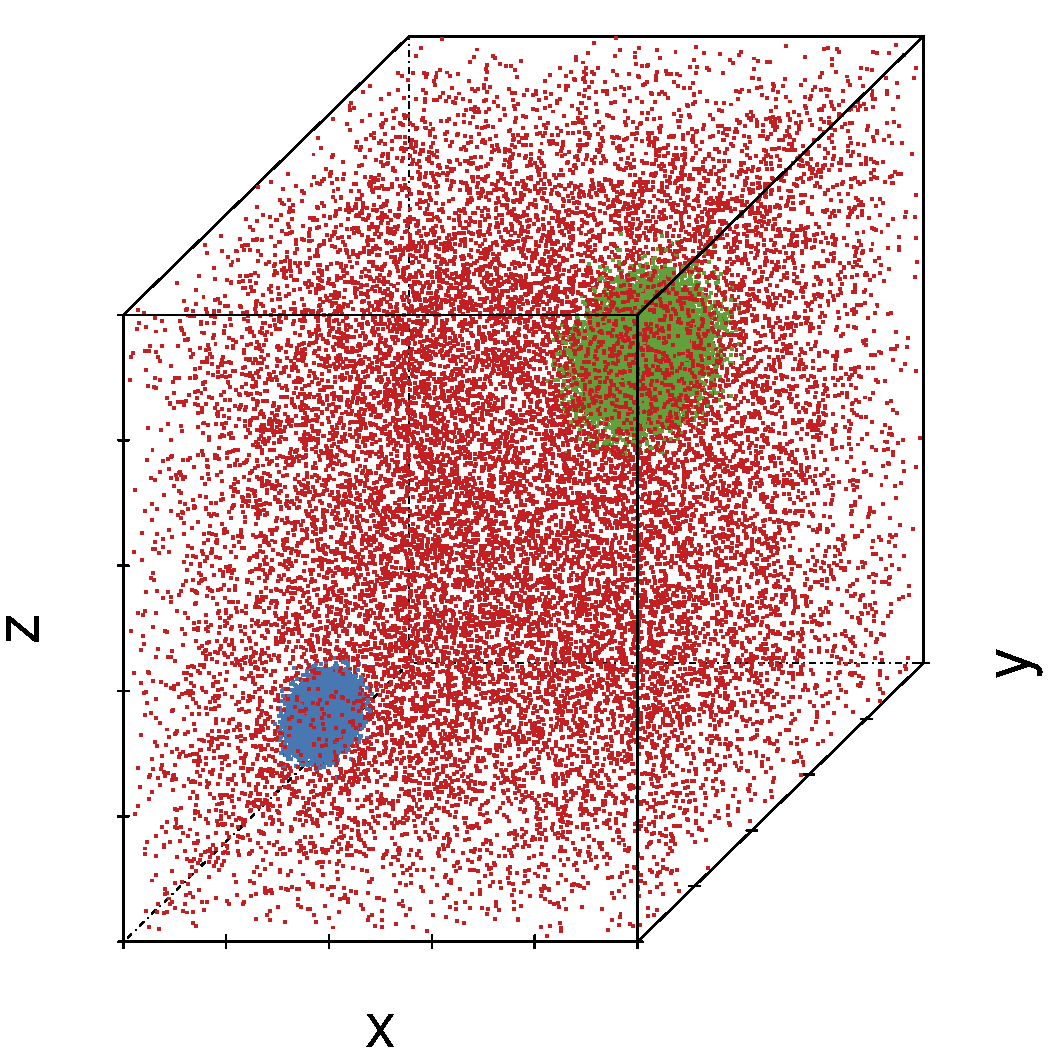
\includegraphics[width=\textwidth]{3/img/datasetplot_ferdosi_2_60000.pdf}
	\caption{Set \ferdosiTwo}
	\label{fig:3:simulated:datasets:ferdosi2}
\end{subfigure}	
\begin{subfigure}{0.23\textwidth}
	\centering
	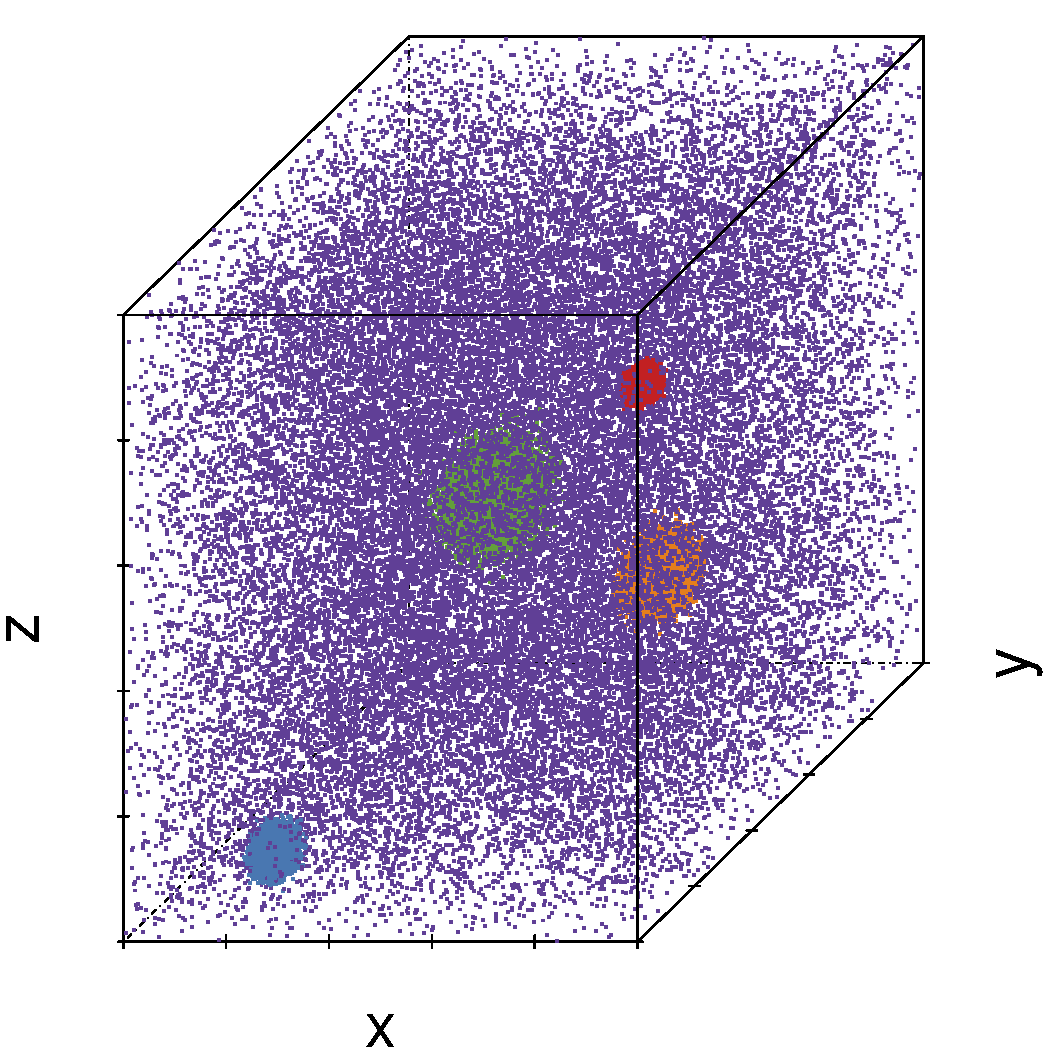
\includegraphics[width=\textwidth]{3/img/datasetplot_ferdosi_3_120000.pdf}
	\caption{Set 3}
	\label{fig:3:simulated:datasets:ferdosi3}
\end{subfigure}	
% Ferdosi Set 4
\begin{subfigure}{0.23\textwidth}
	\centering
	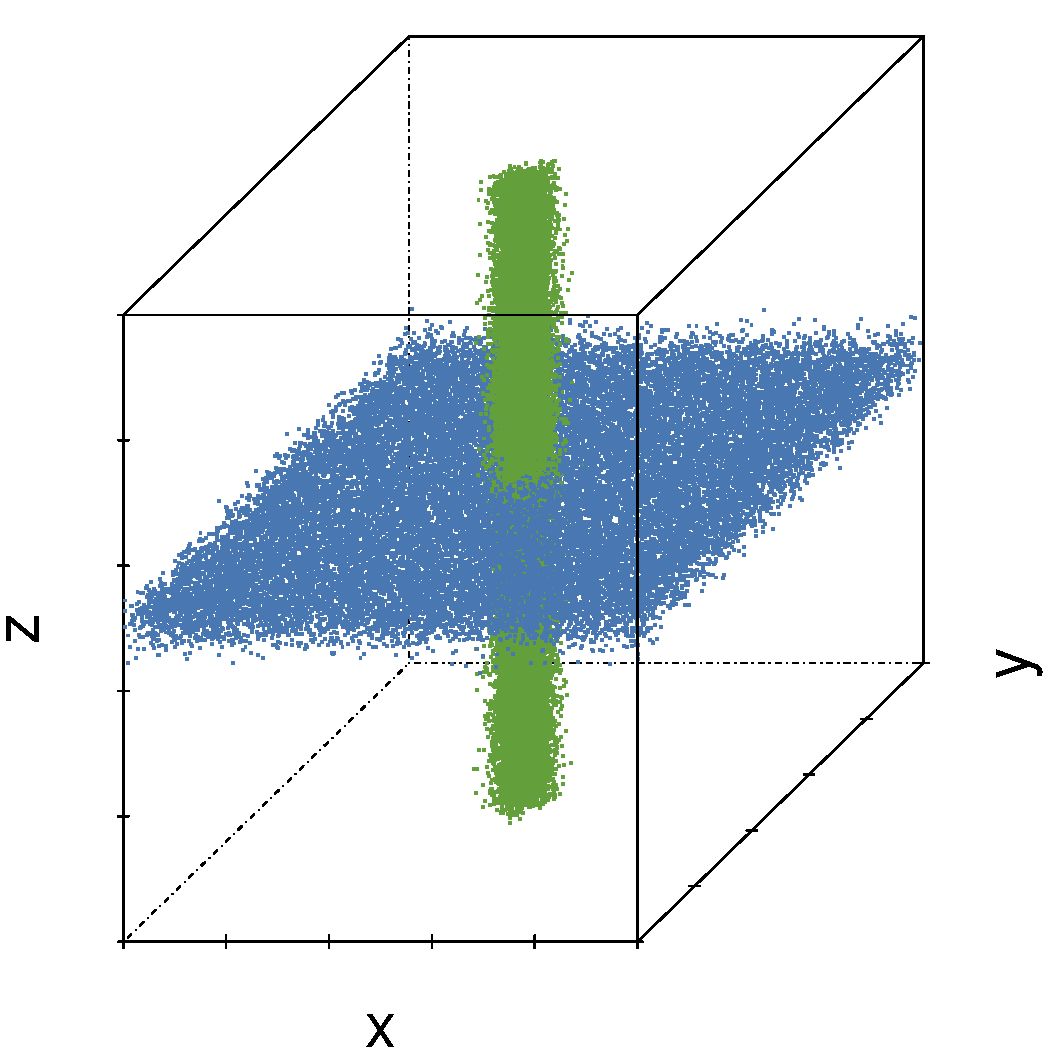
\includegraphics[width=\textwidth]{3/img/datasetplot_ferdosi_4_60000.pdf}
	\caption{Set 7}
	\label{fig:3:simulated:datasets:ferdosi4}
\end{subfigure}
% Baakman 1/3		
\begin{subfigure}{0.23\textwidth}
	\centering
	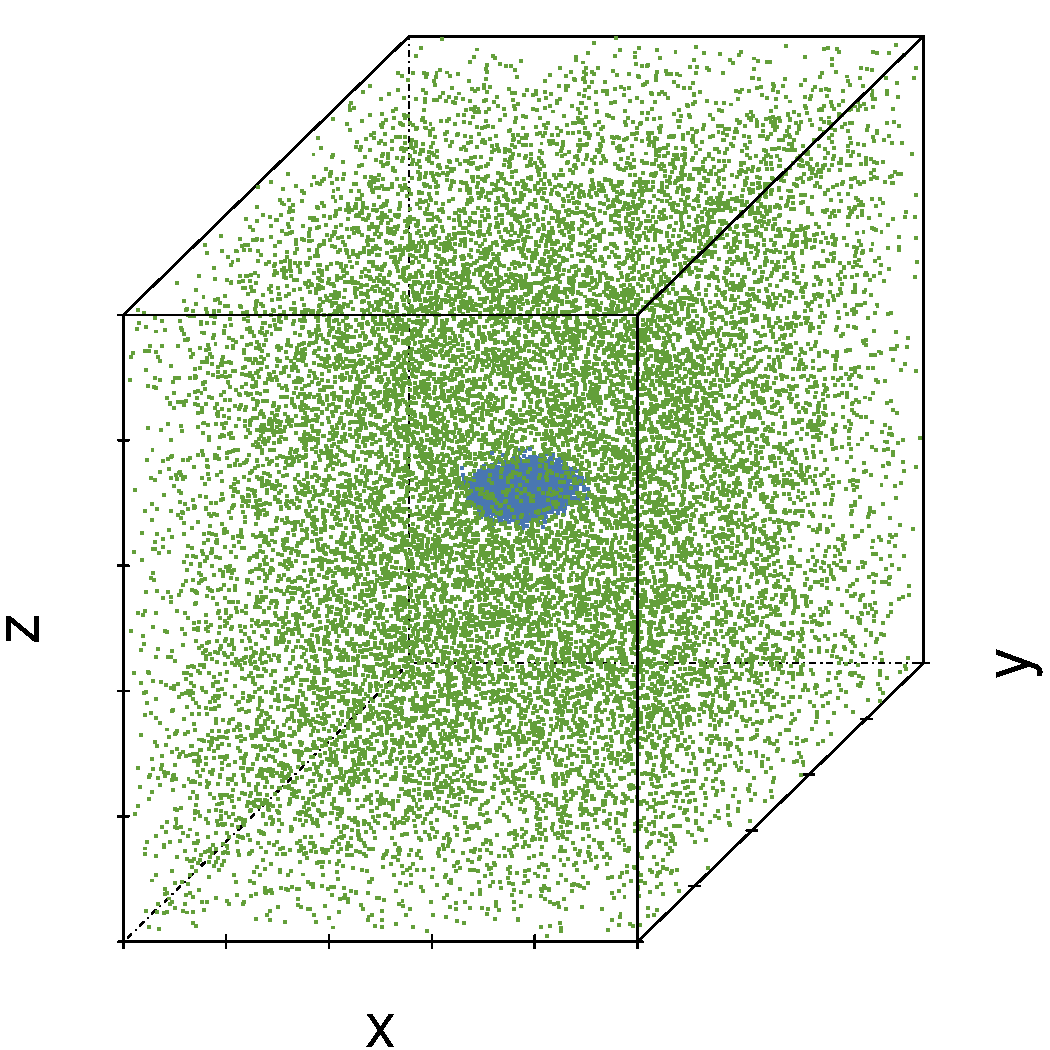
\includegraphics[width=\textwidth]{3/img/datasetplot_baakman_1_60000.pdf}
	\caption{Set 4}
	\label{fig:3:simulated:datasets:baakman1}
\end{subfigure}
\begin{subfigure}{0.23\textwidth}
	\centering
	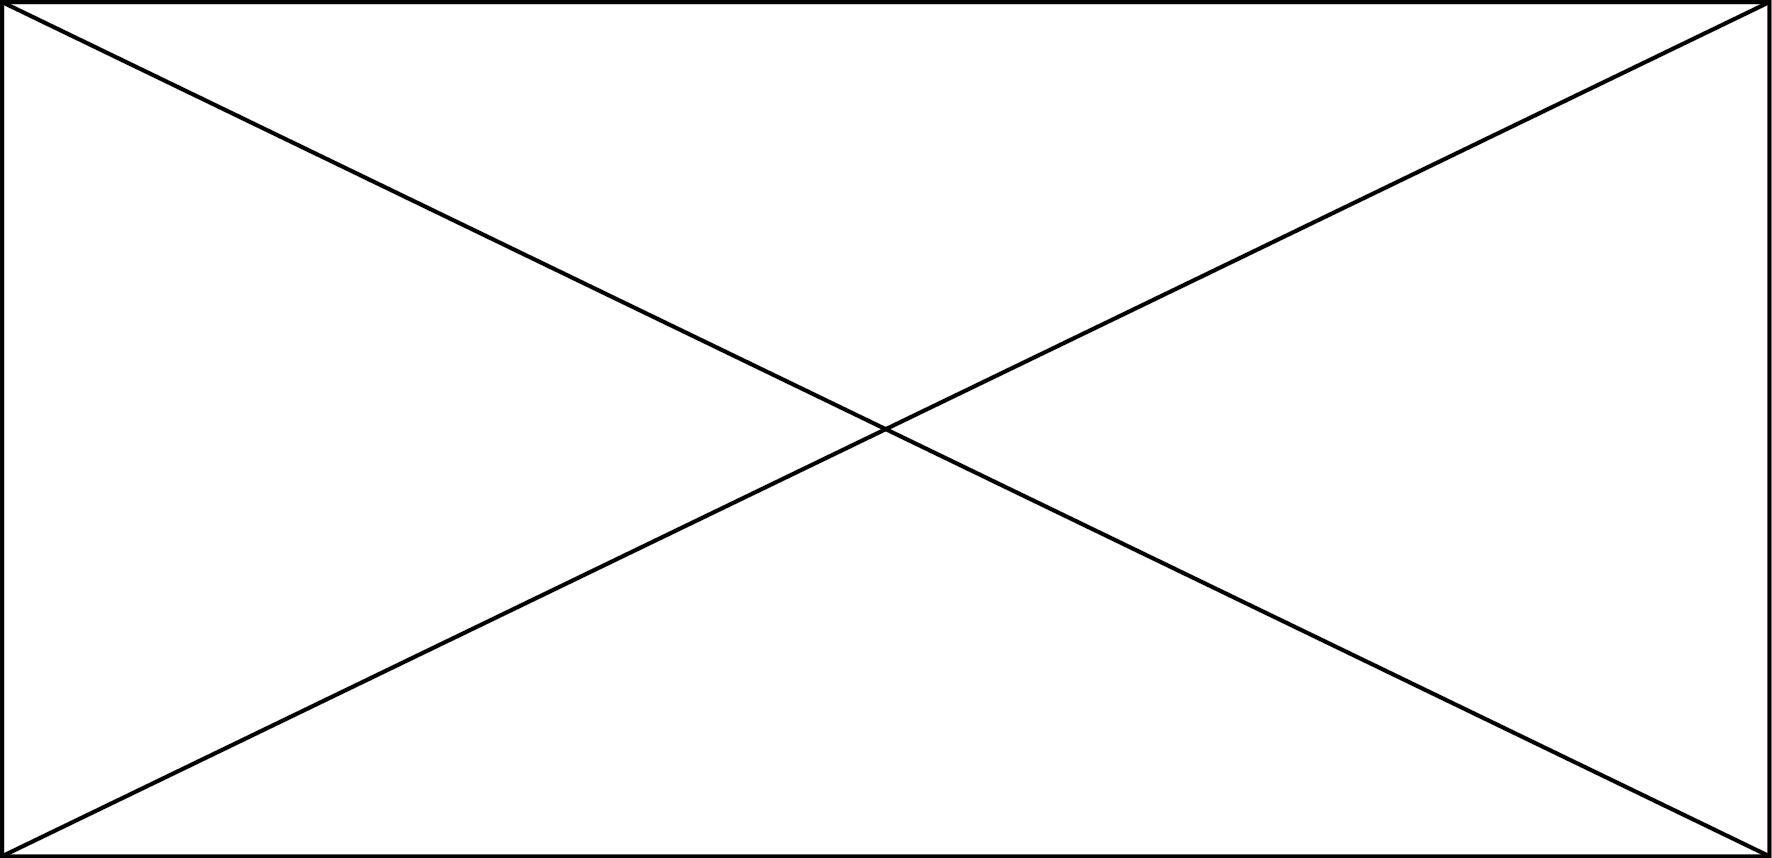
\includegraphics[width=\textwidth]{img/missingfigure.png}
	\caption{Set 5}
	\label{fig:3:simulated:datasets:baakman2}
\end{subfigure}	
\begin{subfigure}{0.23\textwidth}
	\centering
	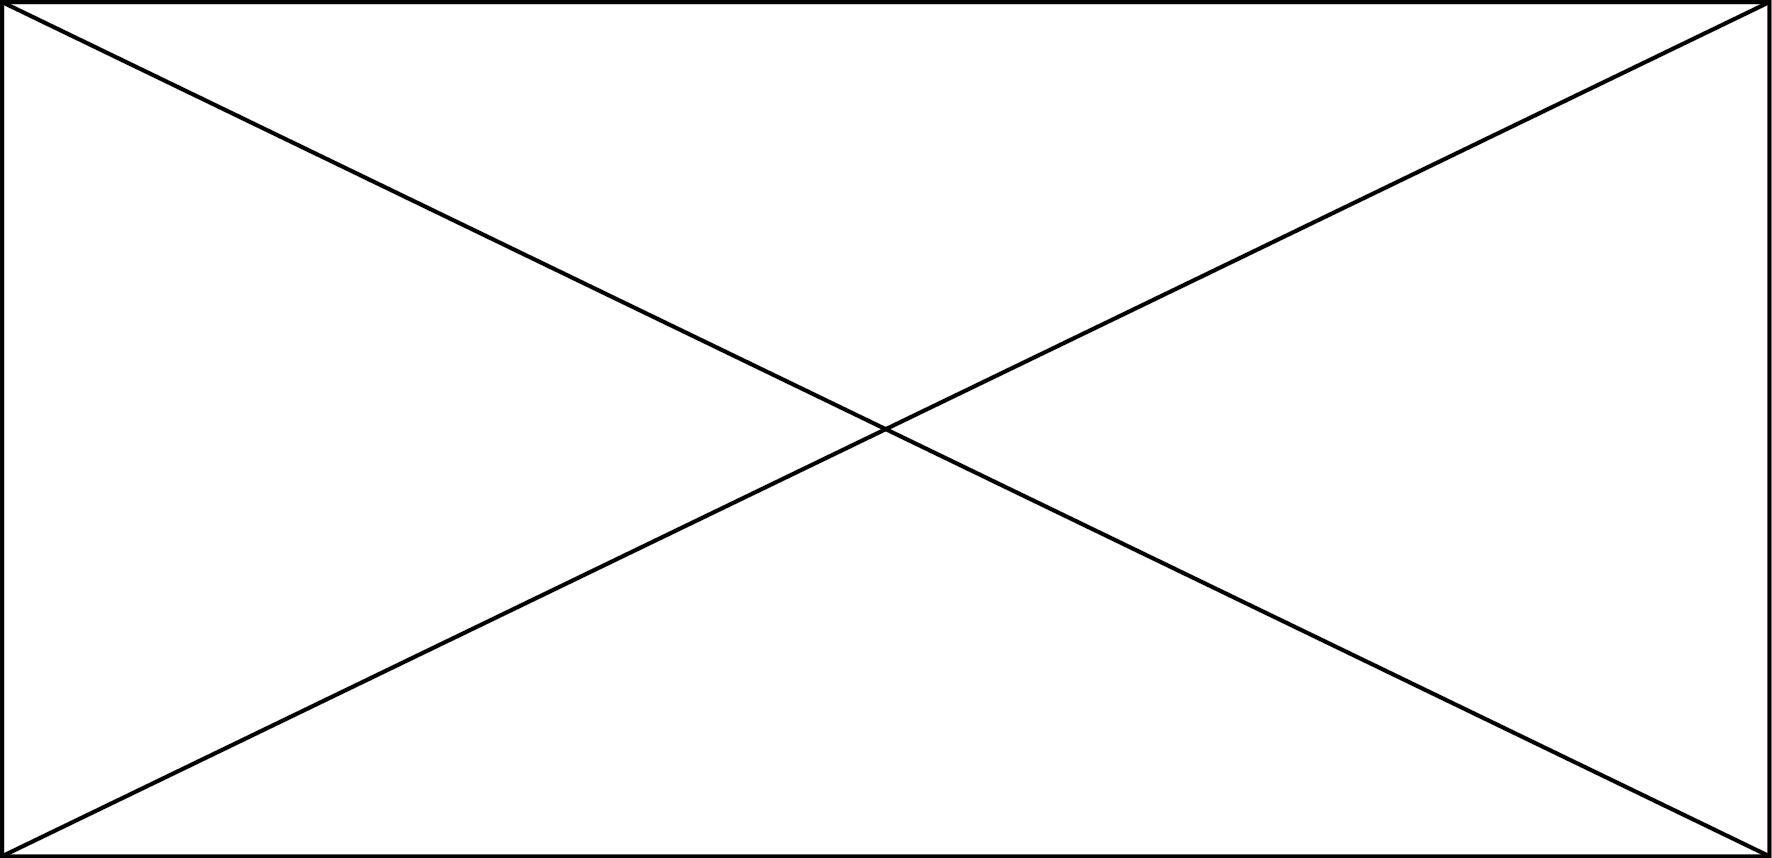
\includegraphics[width=\textwidth]{img/missingfigure.png}
	\caption{Set 6}
	\label{fig:3:simulated:datasets:baakman3}
\end{subfigure}			
% Ferdosi 5
\begin{subfigure}{0.23\textwidth}
	\centering
	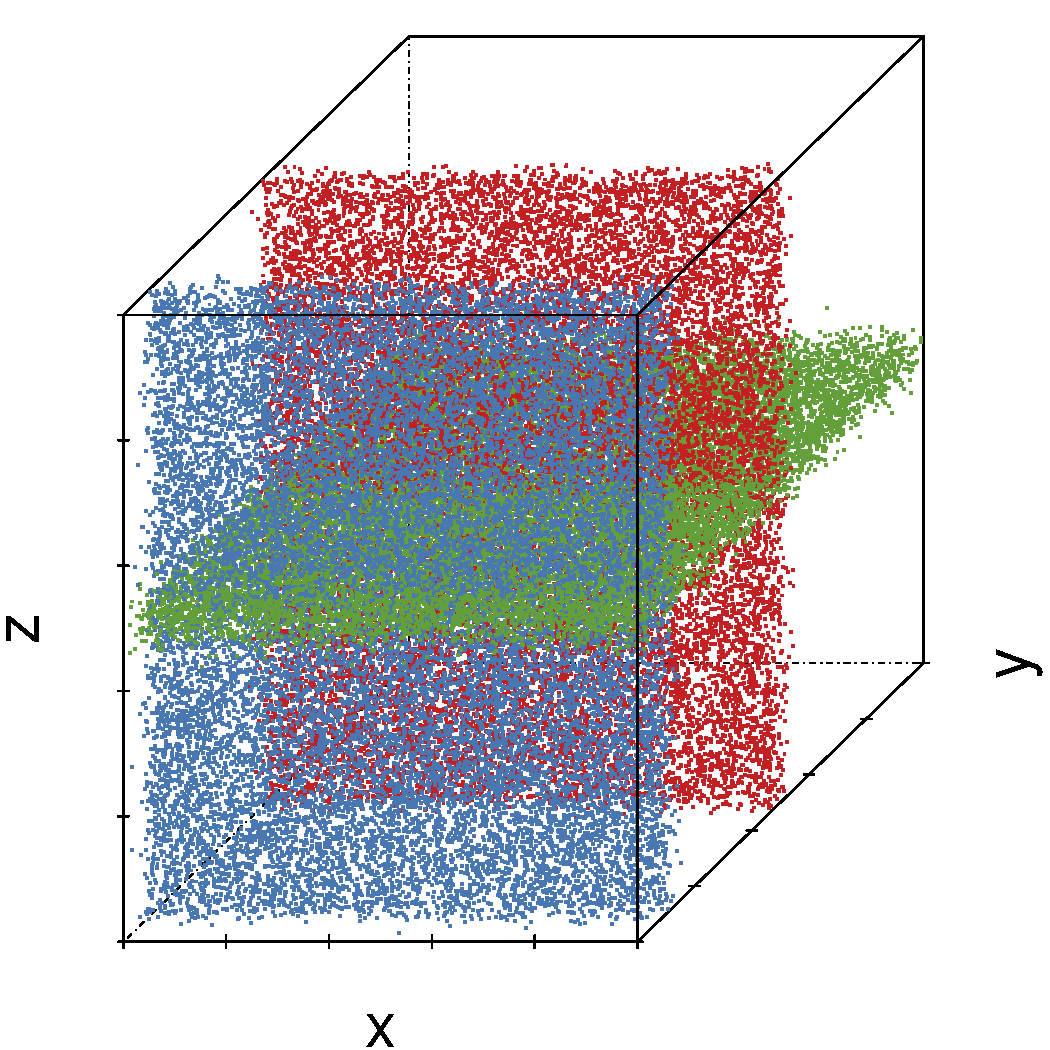
\includegraphics[width=\textwidth]{3/img/datasetplot_ferdosi_5_60000.pdf}
	\caption{Set 8}
	\label{fig:3:simulated:datasets:ferdosi5}
\end{subfigure}				
	\caption{Scatter plot representation of the simulated datasets defined in \cref{tab:3:simulated:datasets}. }
	\label{fig:3:simulated:datasets}
\end{figure*}

\begin{table*}
	\centering
	%!TEX root = ../paper.tex

\begin{tabular}{@{}clcl@{}}
\toprule
Set 		& Component					& Fraction 				& Distribution\\
\midrule
1 			& Trivariate Gaussian 1		& $\rfrac{2}{3}$		& $(x, y, z) \sim \gaussDist{[50, 50, 50]}{\diag(30)}$\\
~ 			& Uniform random background	& $\rfrac{1}{3}$		& $(x, y, z) \sim \uniformDist{[0, 0, 0]}{[100, 100, 100]}$\\
\hline
2 			& Trivariate Gaussian 1		& $\rfrac{1}{3}$		& $(x, y, z) \sim \gaussDist{[25, 25, 25]}{\diag(5)}$\\
~ 			& Trivariate Gaussian 2		& $\rfrac{1}{3}$		& $(x, y, z) \sim \gaussDist{[65, 65, 65]}{\diag(20)}$\\
~ 			& Uniform random background	& $\rfrac{1}{3}$		& $(x, y, z) \sim \uniformDist{[0, 0, 0]}{[100, 100, 100]}$\\
\hline
3 			& Trivariate Gaussian 1 	& $\rfrac{1}{6}$		& $(x, y, z) \sim \gaussDist{[24, 10, 10]}{\diag(2)}$\\
~ 			& Trivariate Gaussian 2 	& $\rfrac{1}{6}$		& $(x, y, z) \sim \gaussDist{[33, 70, 40]}{\diag(10)}$\\
~ 			& Trivariate Gaussian 3 	& $\rfrac{1}{6}$		& $(x, y, z) \sim \gaussDist{[90, 20, 80]}{\diag(1)}$\\
~ 			& Trivariate Gaussian 4 	& $\rfrac{1}{6}$		& $(x, y, z) \sim \gaussDist{[60, 80, 23]}{\diag(5)}$\\
~ 			& Uniform random background	& $\rfrac{1}{3}$		& $(x, y, z) \sim \uniformDist{[0, 0, 0]}{[100, 100, 100]}$\\
\hline
4 			& Wall-like structure 1 	& $\rfrac{1}{2}$		& $(x, z) \sim \uniformDist{[0, 0]}{[100, 100]}$, $(y) \sim \gaussDist{5}{5}$\\
~ 			& Filament-like structure 	& $\rfrac{1}{2}$		& $(x, y) \sim \gaussDist{[50, 50]}{\diag(5)}$, $(z) \sim \uniformDist{0}{100}$\\
\hline
5 			& Wall-like structure 1 	& $\rfrac{1}{3}$		& $(x, z) \sim \uniformDist{[0, 0]}{[100, 100]}$, $(y) \sim \gaussDist{10}{5}$\\
~ 			& Wall-like structure 2 	& $\rfrac{1}{3}$		& $(x, y) \sim \uniformDist{[0, 0]}{[100, 100]}$, $(z) \sim \gaussDist{50}{5}$\\
~ 			& Wall-like structure 3		& $\rfrac{1}{3}$		& $(x, z) \sim \uniformDist{[0, 0]}{[100, 100]}$, $(y) \sim \gaussDist{50}{5}$\\
\bottomrule
\end{tabular}
	\caption{The simulated datasets used to test the estimators. The column `Fraction' indicates for each component of the dataset which fraction of the total number of points of the data set is part of that component. \gaussDist{\varMean}{\varCovarianceMatrix} denotes a Gaussian distribution with mean \varMean and covariance matrix \varCovarianceMatrix. A diagonal matrix with the value $x$ on the diagonal is represented as $\diag(x)$. \uniformDist{a}{b} denotes a uniform distribution with its minimum and maximum set to $a$ and $b$, respectively. The colors shown in the second column correspond with the colors used for these components of the data set throughout the paper.} 	
	\label{tab:3:simulated:datasets}
\end{table*}

%Data Set 1
	Dataset \ferdosiOne, shown in \cref{fig:3:simulated:datasets:ferdosi1}, is the most simple set in this group. It is an unimodal Gaussian distribution with random noise added. 

%Data Set 2
	The second dataset, depicted in \cref{fig:3:simulated:datasets:ferdosi2}, contains two Gaussian distributions with different covariance matrices and uniform noise. The means and covariance matrices of the Normal distributions are such that the two distributions are very unlikely to overlap. 

%Data Set 3
	Dataset 3, represented in \cref{fig:3:simulated:datasets:ferdosi3}, consists of four different normal distributions and uniformly distributed noise. The four Gaussian distributions are placed in such a way that it is unlikely that among them any overlap occurs.

%Data Set 4
	\Cref{fig:3:simulated:datasets:ferdosi4} illustrates dataset 4. This set consists of a horizontal wall-like structure and a vertical filament-like structure. 

%Data Set 5
	The fifth dataset, shown in \cref{fig:3:simulated:datasets:ferdosi5}, contains three intersecting walls. For each point in these walls its position in two of the three dimensions is drawn from a uniform distribution, the third coordinate is sampled from a Gaussian distribution.


%Expectations for the datasets
We expect comparable performance from all estimators on dataset one through three, as other than the randomly sampled noise these sets only contain data sampled from a Gaussian distribution with a diagonal covariance matrix. Which results in an equal spread of the data in all dimensions for the non-noise data. Dataset four and five are clearly spread more in one dimension than in others, thus we expect the shape adaptive estimator to outperform the MBE estimator.

%Conclusion
The increasing complexity of these datasets allows us to investigate the performance of the classifier on simple situations, one cluster of data with some noise, to complex density fields that should better approximate real world data. The advantage of using simulated data is that the true densities of the data points are known, which allows us to test how well the different methods estimate the densities.				

	\subsubsection*{Real World Datasets}
	\todo[inline]{Iets over real world data}

\subsection{Error Measures}
\label{ss:3:errorMeasures}
%!TEX root = ../paper.tex
To quantify the performance of the estimators on the simulated datasets we use the Mean Squared Error (MSE):
\begin{equation*}
	\varMSE{\varEstimatedDensityFunction{\bullet}} = \frac{1}{\varNumPatterns} \sum_{i = 0}^{\varNumPatterns} {\left(\varEstimatedDensityFunction{\varPattern{i}} - \varDensityFunction{\varPattern{i}} \right)}^2.
\end{equation*}
\todo[inline]{Iets over het quantificeren van de resultaten op real world data.}

